\documentclass[11pt]{report}

\usepackage[T1]{fontenc}
\usepackage[polish]{babel}
\usepackage{mathptmx}
\usepackage[utf8]{inputenc}
\usepackage{lmodern}
\usepackage{enumitem}
\usepackage{setspace}
\usepackage{advdate}
\usepackage{graphicx}
\usepackage{subfiles}
\usepackage[toc,page]{appendix}
\usepackage{comment}
 
\newcommand{\LabNum}{1}
\setcounter{chapter}{\LabNum}
\usepackage[none]{hyphenat}
\selectlanguage{polish}
\usepackage[left=2.5cm,top=2.5cm,right=2.5cm,bottom=2.5cm,bindingoffset=0.5cm]{geometry}

\begin{comment}
LATEX 101:

Pogrubiony - \textbf{gruby}
Pochylony  - \textit{pochyły}
Nowa linia - \\
Nowa strona - \newpage
Bez wcięcia - \noindent

LISTA:
\begin{itemize}
    \item coś
    \item tam
\end{itemize}

TABELA:
Tu jest spoko narzędzie do robienia tego
https://www.tablesgenerator.com/latex_tables

RYSUNEK:
\begin{figure}[h!]
  \centering
    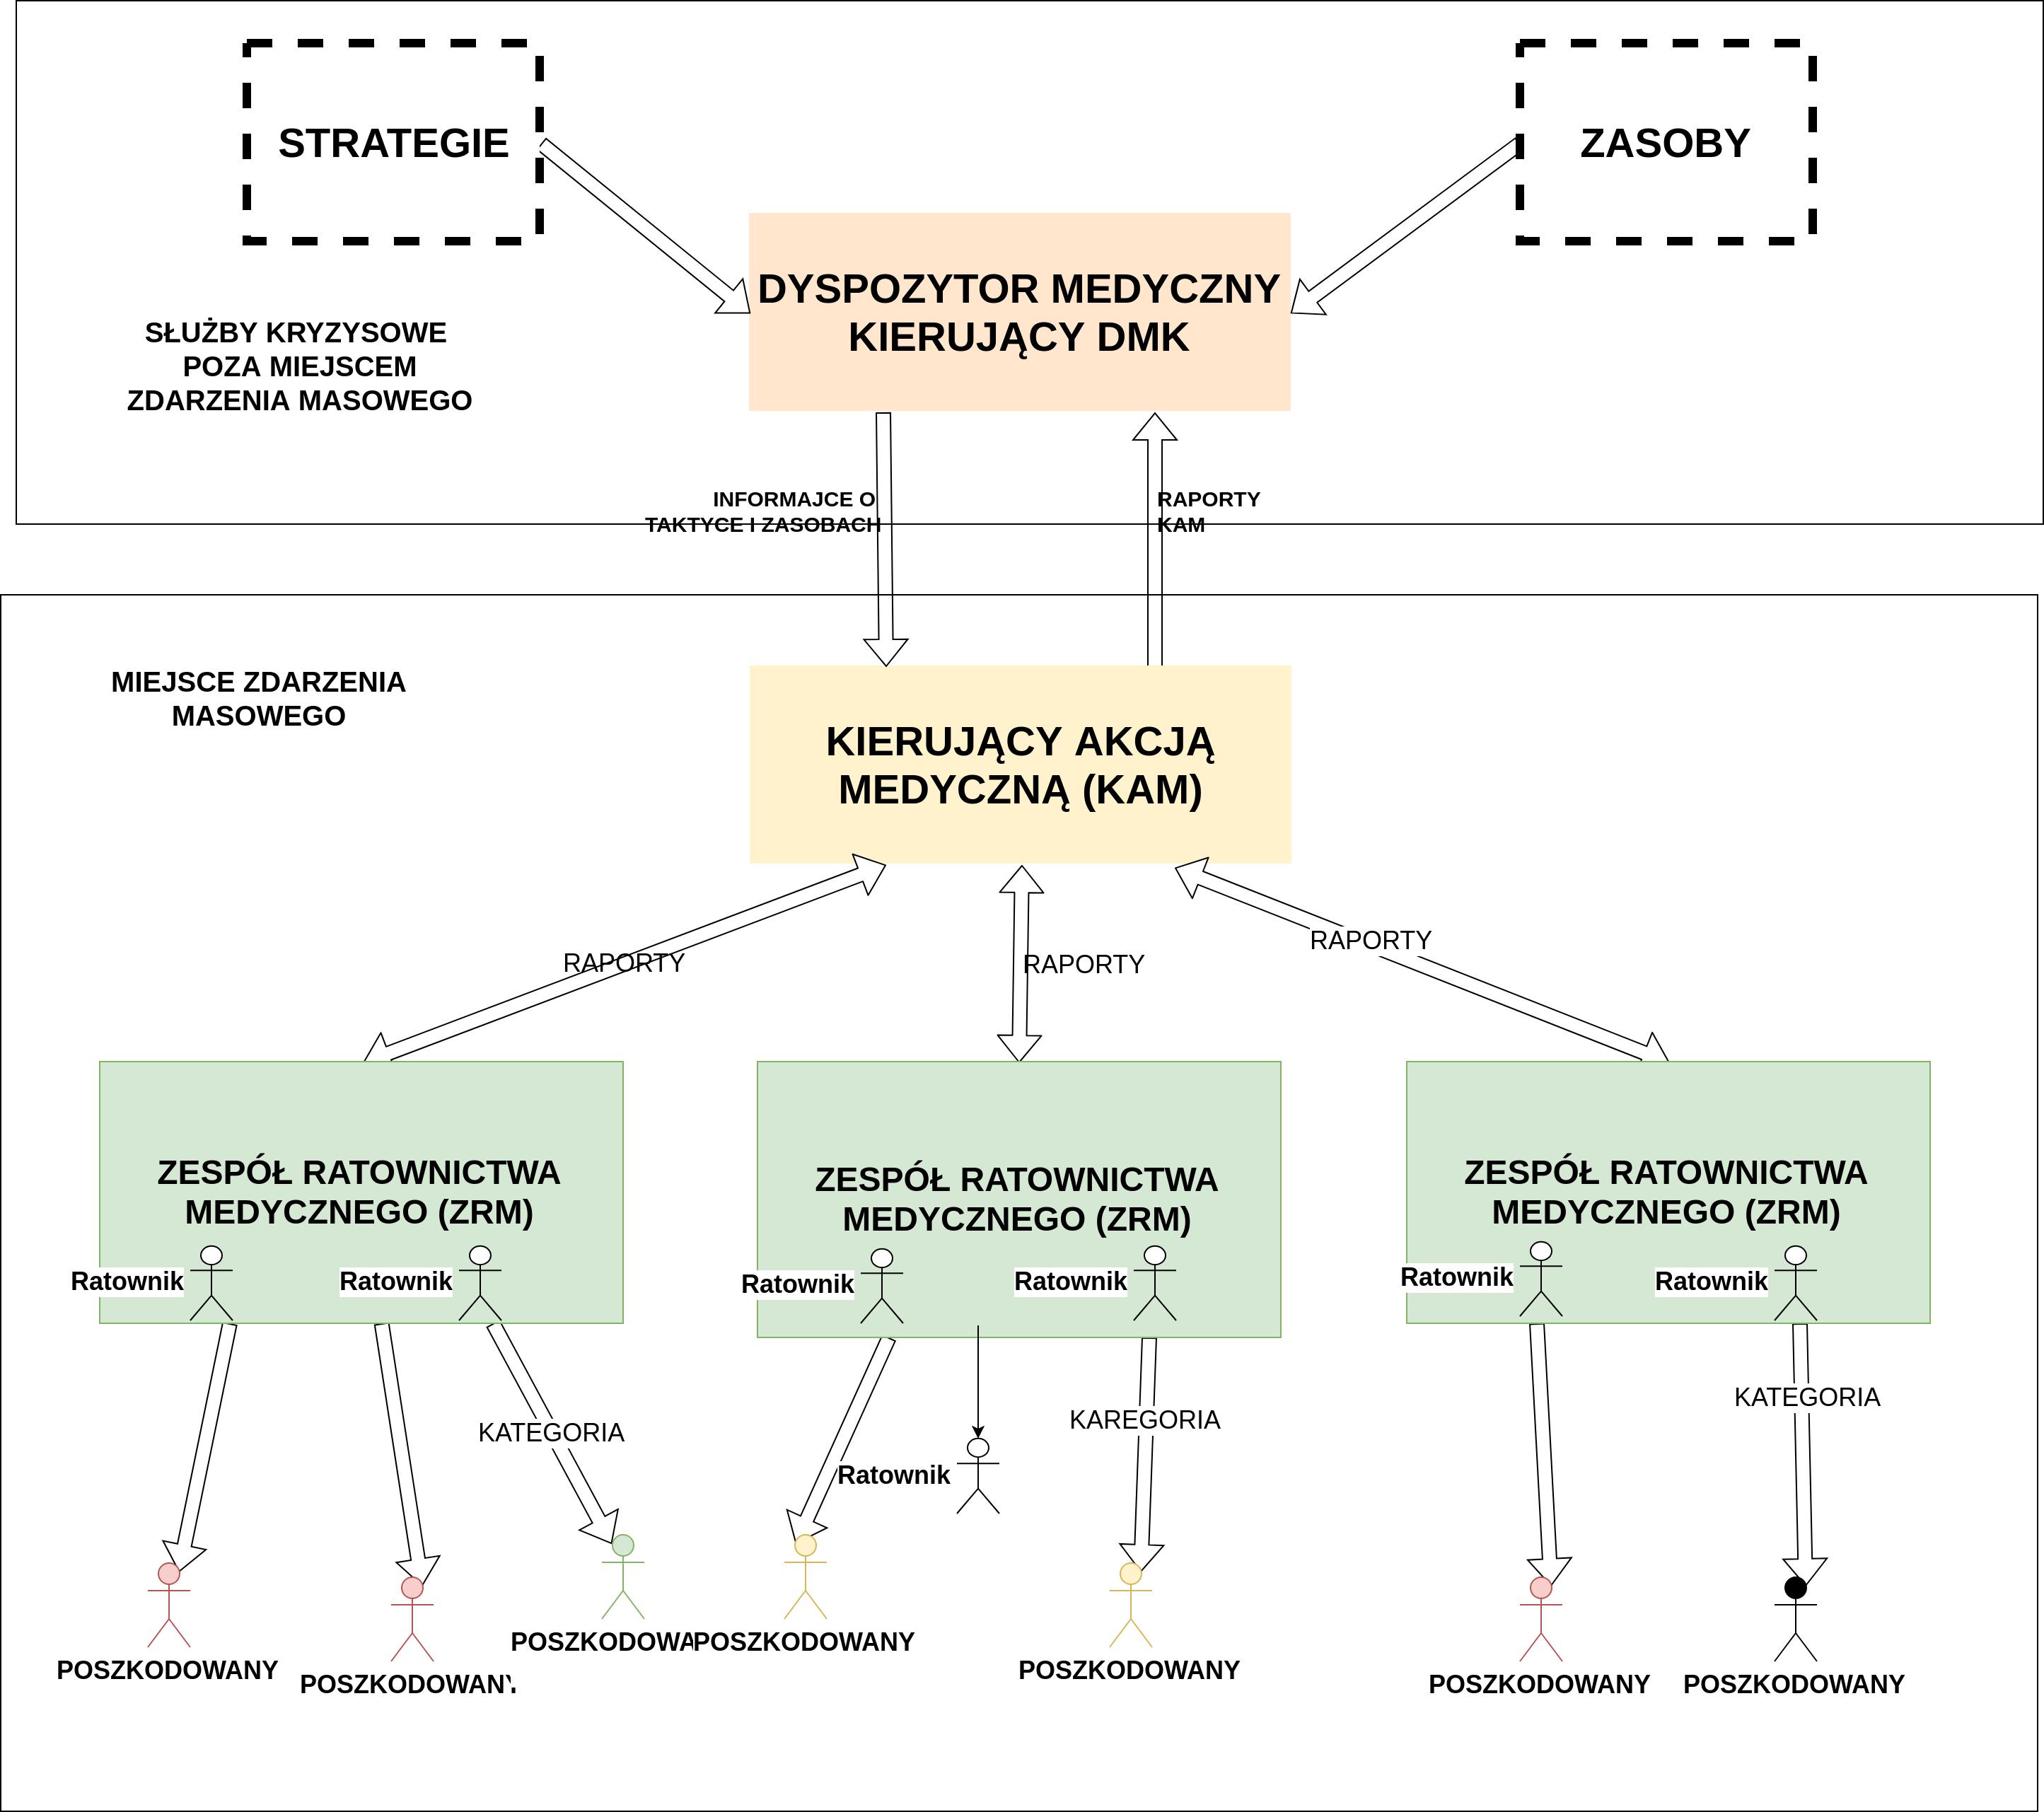
\includegraphics[width=0.95\textwidth]{img/hierarchy.png}
  \caption{Organizacja działania podczas zdarzeń masowych} -> podpis
  \label{fig:org}                                       -> odniesienie się do rysunku
\end{figure}

ODNIESIENIA:
Żeby odnieść się do rysunku trzeba dać \ref{fig:org} gdzie fig:name to labelka którą czemuś daliśmy

CUDZYSŁÓW:
dawać '' a nie ""
Jeśli jest jakiś znak który coś psuje a jest potrzebny to można go zeskejpować np. \%
\end{comment}



\begin{document}
\begin{titlepage}
   \begin{center}
        \vspace*{1cm}
        \Huge
        \textbf{Triage}
    
    \vspace{0.5cm}
    Projekt Zespołowy
    
    \vspace{1.5cm}
    
    \normalsize
    \textbf{
        Jan Niewiarowski,  210828\\
        Adrian Winiarski, 225948\\
        Szymon Klimczuk, 221521\\
        Oliwier Salamon, 225990\\
        Jakub Sokołowski, 226080\\
        Mateusz Skowronek, 225945
    }
    
    \normalsize
    \textbf{
    \newline
    \newline
        Termin zajęć: poniedziałek 14:15\\
        Prowadzący: dr inż. Jan Nikodem\\
    }
    \vfill
    
    
    \vspace{0.8cm}
    
    
\includegraphics[width=0.2\textwidth]{img/pwr-logo.png}
    
    Wydział Elektroniki\\
    Informatyka\\
    Inżynieria Internetowa\\
    2019
 
   \end{center}
\end{titlepage}
\tableofcontents
\newpage
\section{Wymagania projektu}
Projekt ma za zadanie stworzenie aplikacji wspomagającą procedure \textit{triage}. Procedura ta, nazywana również 'segregacją medyczną', stosowana podczas tzw. zdarzeń masowych (takich jak wypadki w transporcie lotniczym, czy ataki terrorystyczne) w których zapotrzebowanie na pomoc medyczną znacznie przekracza możliwości jej udzieleni. Polega na wyznaczaniu kategorii leczniczo-transportowych poszkodowanych w zależności od stopnia obrażeń oraz rokowania. 

\noindent
W Polsce obecnie wykorzystywanych jest kilka modeli triage'u:
\begin{itemize}
    \item{
        oparty na systemie  \textit{START- Simple Triage and Rapid Treatment} oraz jego modyfikacji pediatrycznej \textit{JumpSTART}
    }
    \item{
        oparty na ocenie pacjentów na podstawie skali ciężkości urazów-  \textsc{TRTS}\textit{- Triage Revised Trauma Score}, \textsc{ISS}- \textit{Injury Severity Score}, \textit{BTTR - Baxt Trauma Triage Rule}
    }
    \item {
        Triage taktyczny – odwrócony – w ramach \textsc{TCCC}-\textit{Tactical Combat Casualty Care}.
    }
\end{itemize}
Najczęściej poszkodowani dzieleni są na cztery priorytet, a więc kolejności udzielania pomocy medycznej oraz transportu. Natychmiastowa – dla poszkodowanych z obrażeniami ciała, które w krótkim czasie doprowadzą do śmierci, a więc będących w stanie bezpośredniego zagrożenia życia. Osoby te powinny otrzymać pomoc w pierwszej kolejności i zostać oznaczone kolorem czerwonym. Pilna – dla poszkodowanych z obrażeniami, których leczenie może zostać odłożone na pewien czas, a więc w chwili badania nie występuje bezpośrednie zagrożenie życia. Osoby te powinny otrzymać pomoc w drugiej kolejności i zostać oznaczone kolorem żółtym. Odroczona – dla poszkodowanych z lekkimi obrażeniami, których życie ani zdrowie nie jest zagrożone nawet podczas długiego oczekiwania na pomoc. Osoby te powinny otrzymać pomoc w trzeciej kolejności i zostać oznaczone kolorem zielonym. Martwi – dla poszkodowanych, u których stwierdzono brak czynności życiowych. U osób tych nie podejmuje się prób ratowania, odstępując od resuscytacji krążeniowo-oddechowej. Osoby te powinny zostać oznaczone kolorem czarnym. W zależności od priorytetu poszkodowani oznaczani są kartami różnego koloru. Na kartach znajdują się dodatkowe informacja umożliwiające zidentyfikowanie poszkodowanego w trakcie przekazywania, transportu i leczenia szpitalnego, stanu poszkodowanego oraz podjętych działań.
\\\\
Segregacja prowadzona niezwłocznie po przybyciu na miejsce zdarzenia podmiotu ratowniczego zwana jest segregacją pierwotną (wstępną). Po wdrożeniu medycznych czynności ratunkowych wobec osób poszkodowanych z grupy o najwyższym priorytecie (czerwonej) należy przejść do drugiego etap triage’u, zwanego segregacją wtórną, czyli ponownej oceny poszkodowanych.
\newpage
\noindent
W Polsce stosowane są różne procedury i zalecenia dotyczące zdarzeń masowych, które definiują sposoby postępowania i łańcuch dowodzenia podczas tych zdarzeń \cite{procedury}. Uproszczony schemat organizacji działań znajduje się na rysunku \ref{fig:org}.
\begin{figure}[h!]
  \centering
    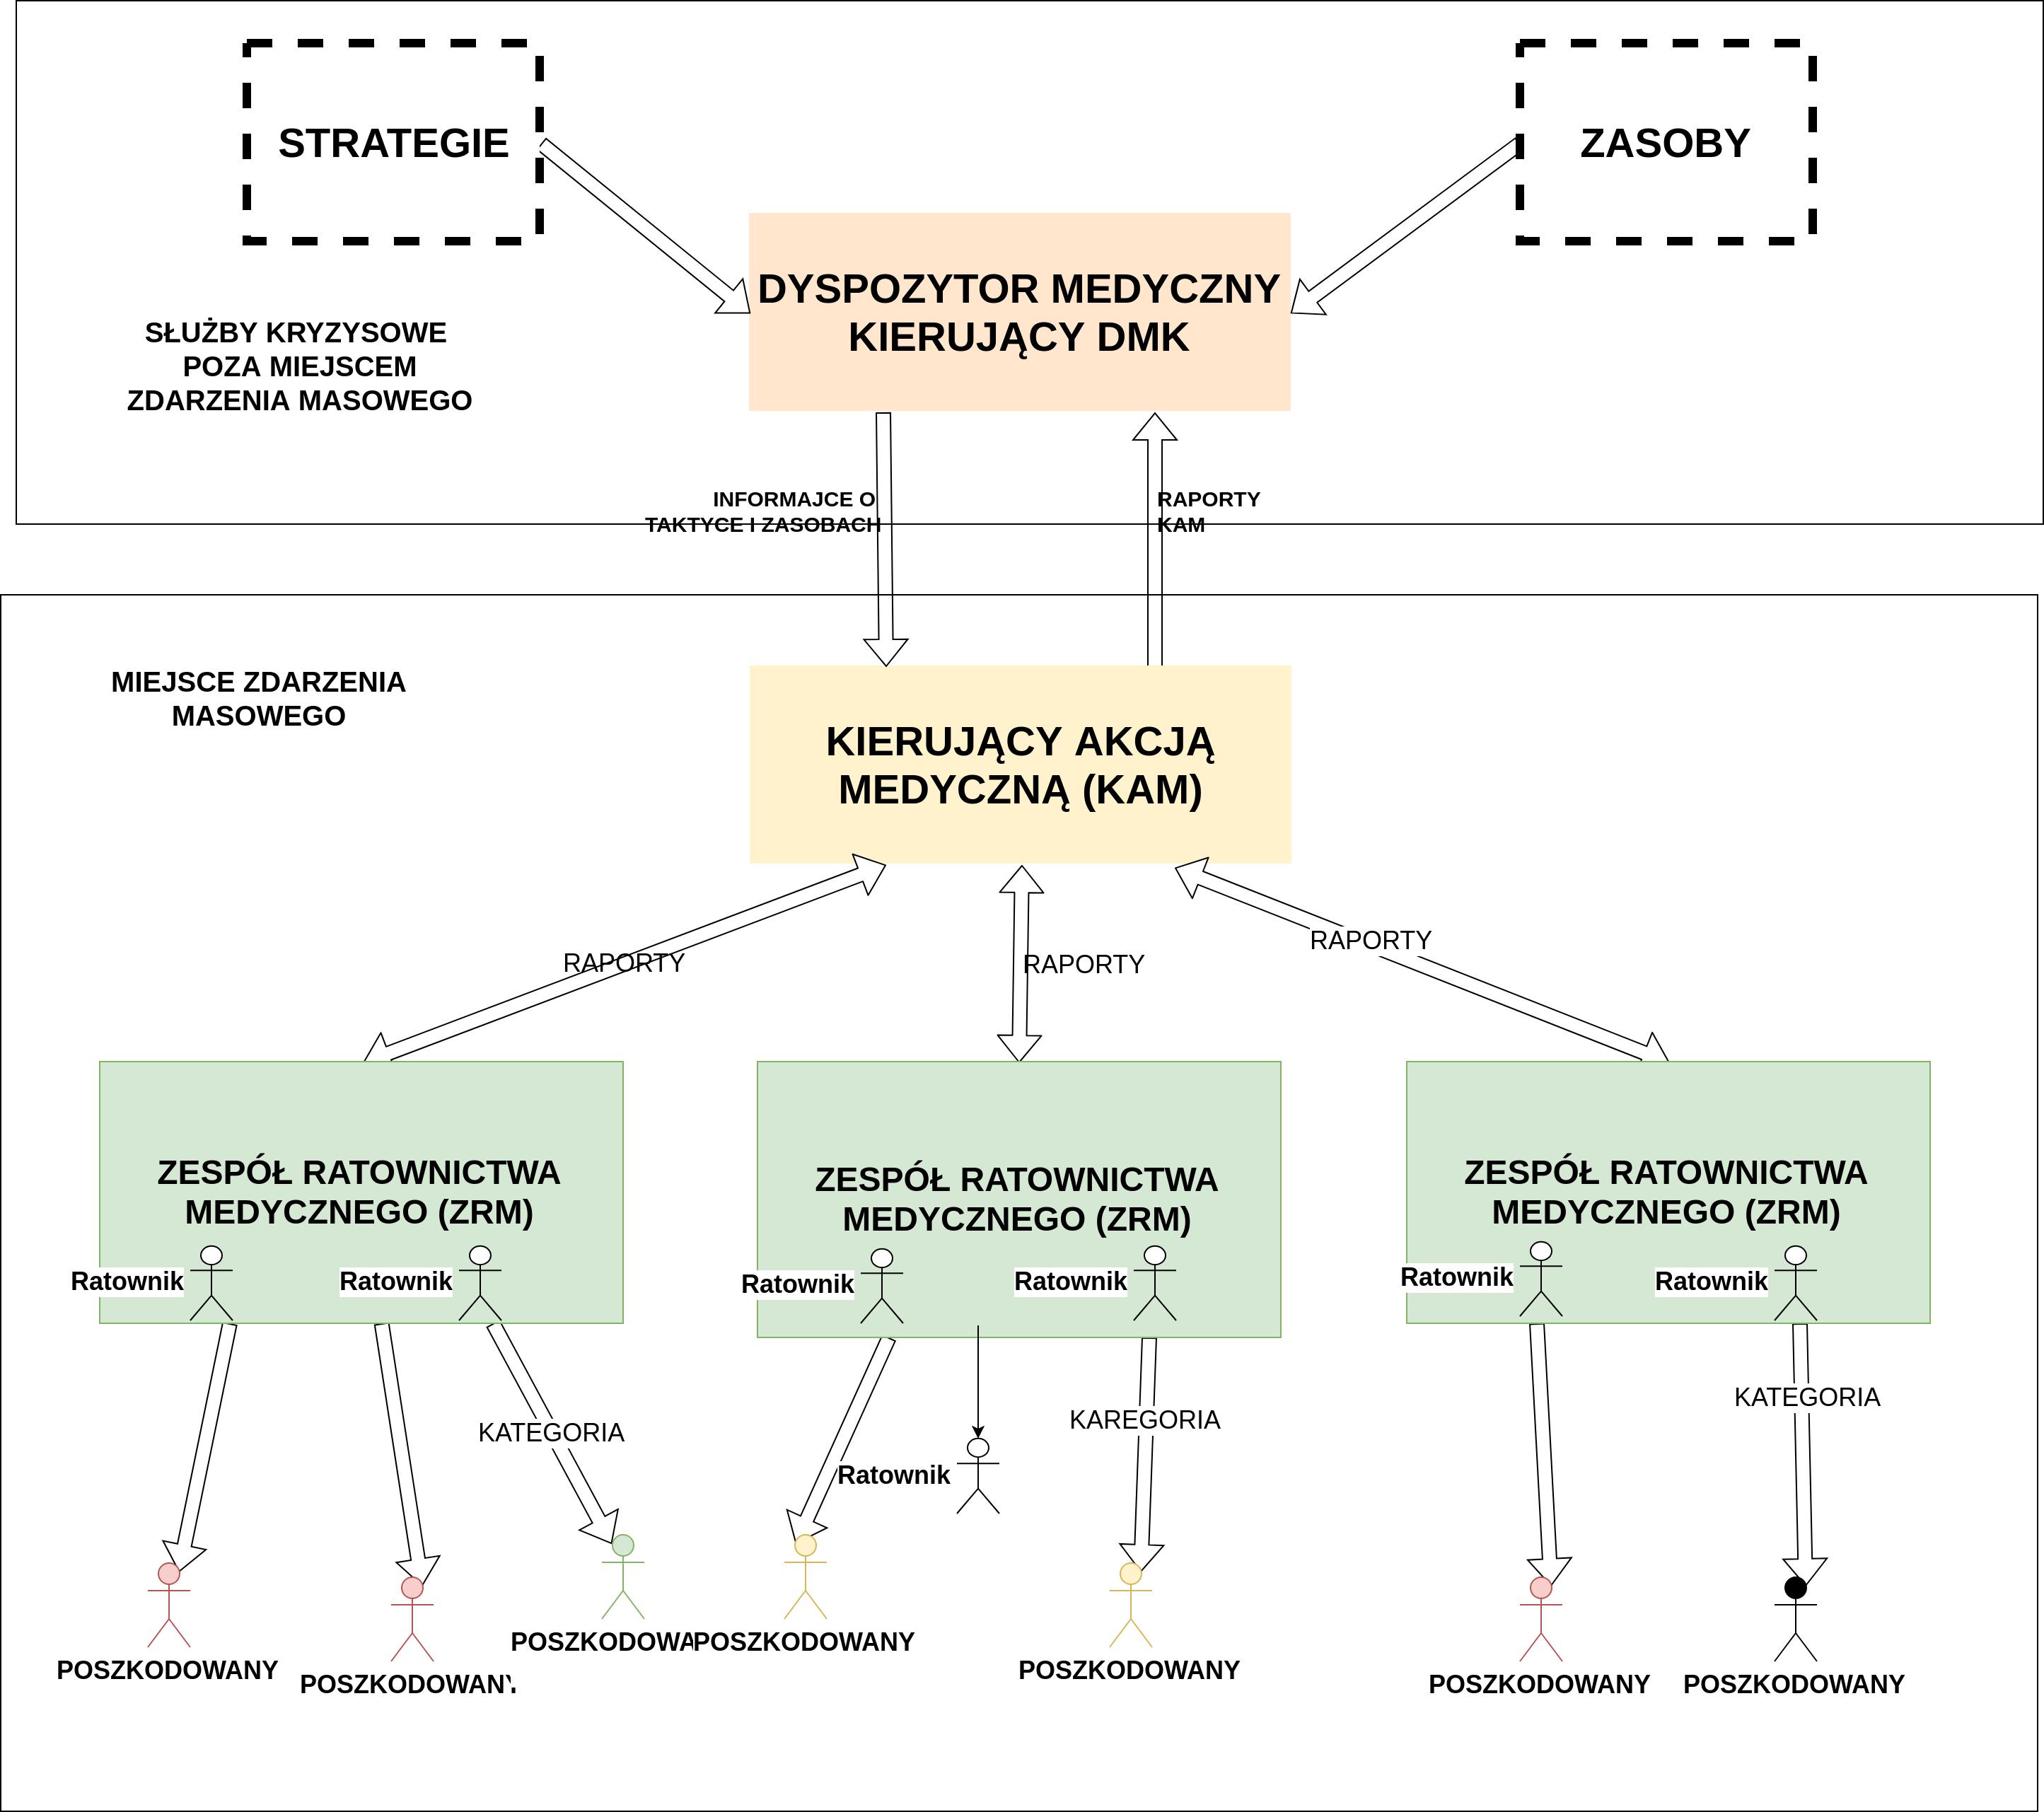
\includegraphics[width=0.95\textwidth]{img/hierarchy.png}
  \caption{Organizacja podczas zdarzeń masowych}
  \label{fig:org}
\end{figure}
\\
Na miejscu zdarzenia znajduje się Kierujący Akcją Medyczną (KAM). Głównym zadaniem KAM jest ustalanie dyslokacji poszkodowanych z grupy czerwonej, w oparciu o stan zdrowia, czas transportu, możliwości ZRM oraz dostępności leczenia specjalistycznego. Do jego obowiązków należy również zbieranie informacji z przebiegu akcji i przekazywanie tych informacji w formie raportów do Dyspozytora Medycznego Kierującego DMK. DMK odpowiada za przyjęcie powiadomienia o wystąpieniu zdarzenia i zakwalifikowanie takiego zdarzenia jako zdarzenie o charakterze mnogim/masowym. W porozumieniu z KAM analizuje zapotrzebowania i dysponuje zasobami.
\newpage
\section{Założenia i architektura systemu}
W ramach projektu zostanie zrealizowany system wspomagający procedure triage, który skupia się na wspomaganiu działań na miejscu zdarzenia masowego. W zaprojektowanym systemie znajdą się następujące elementy:
\begin{itemize}
    \item aplikacja poszkodowanego - czujnik funkcji życiowych
    \item aplikacja członka ZRM
    \item aplikacja KAM
\end{itemize}
Poniższy diagram przedstawia komunikację elementów systemu \ref{fig:arch}
\begin{figure}[h!]
  \centering
    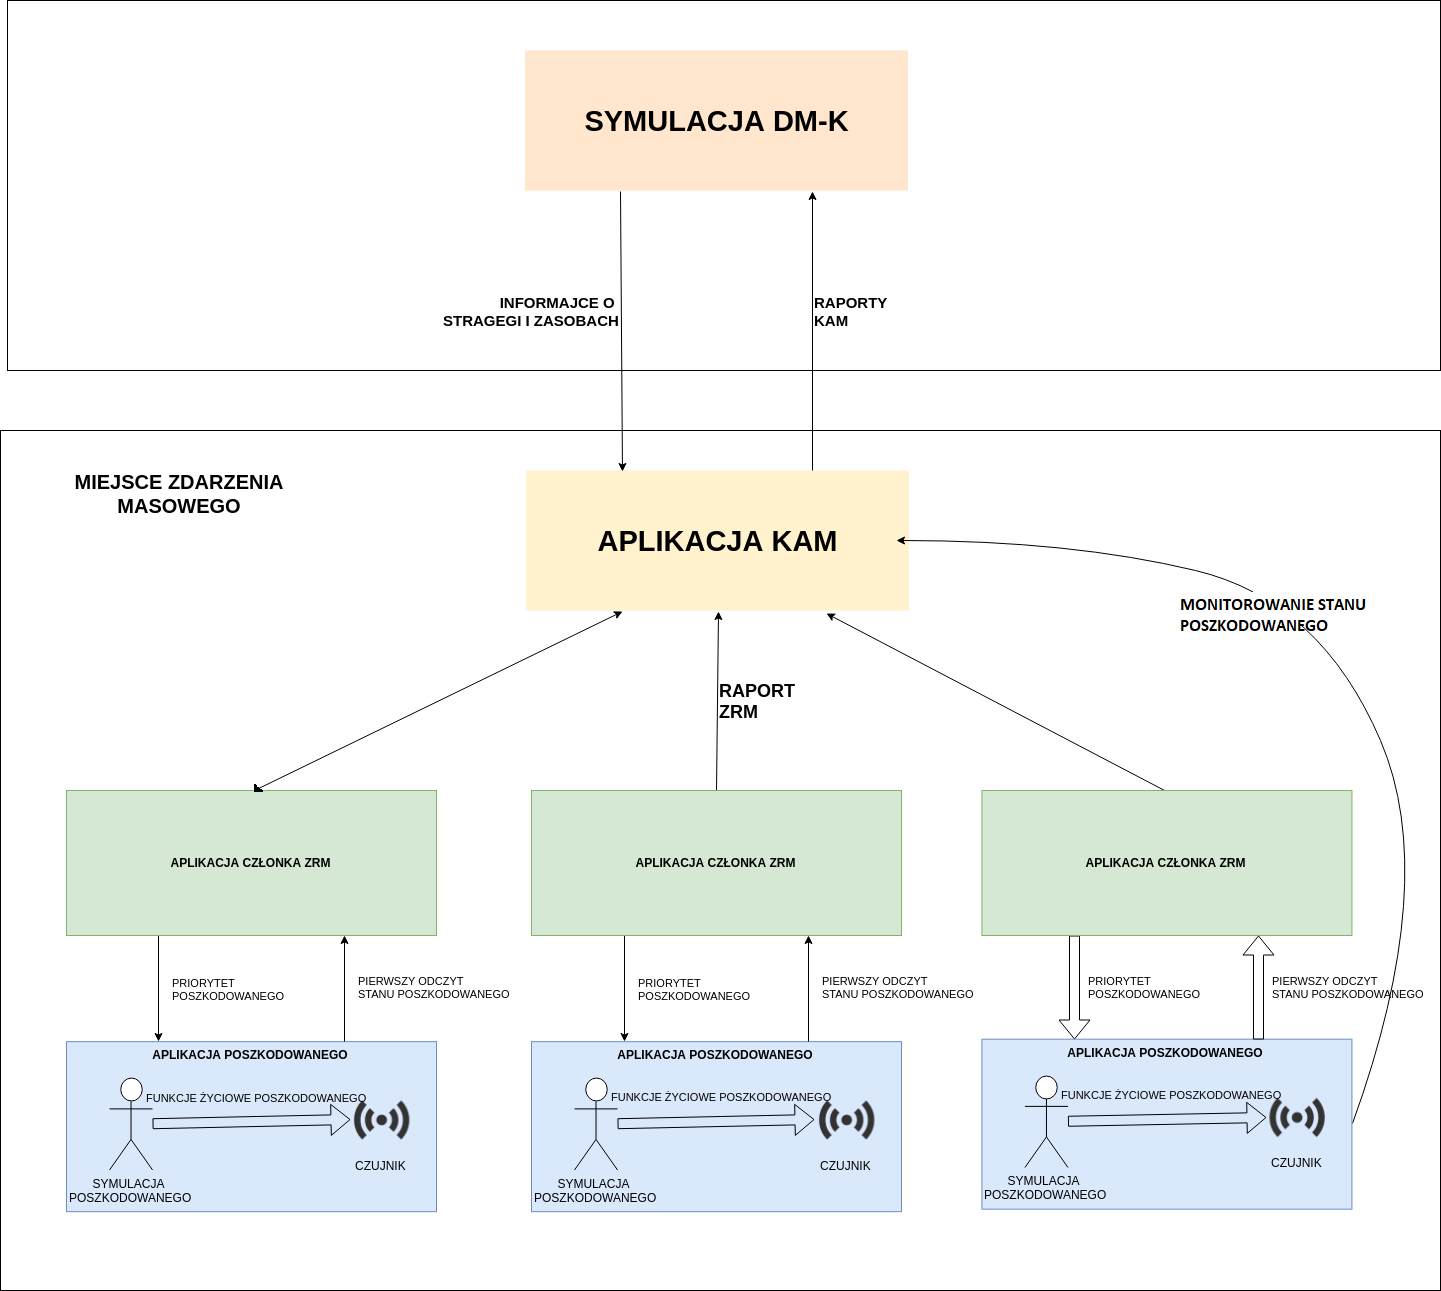
\includegraphics[width=0.95\textwidth]{img/arch.png}
  \caption{Diagram komunikacji}
  \label{fig:arch}
\end{figure}
\newpage
\subsection{Czujnik}
Czujnik odczytuje dane z symulacji pacjenta i transmitować te dane, wraz z danymi o lokalizacji dalej. Dane można transmitować w dwa miejsca w zależnośći od scenariusza - jednorazowo, do aplikacji ZRM- gdy osoba z zespołu ZRM znajduje się w pobliżu poszkodowanego i wykonuje procedure triage lub stale do aplikacji KAM, od momentu zakończeniu działania ratownika.
\noindent
Ratownik nie powinien poświęcać poszkodowanemu więcej niż minutę. Na potrzeby projektu wspomnianym narzędziem wybrany został pulsoksymetr napalcowy.
\noindent
Pulsoksymetr - urządzenie elektroniczne służące do nieinwazyjnego pomiaru saturacji krwi, wykorzystujące pomiar pochłaniania przez tkanki promieniowania 
o dwóch różnych długościach fal metodą pulsoksymetrii. Działa na zasadzie pomiaru pochłaniania przez czerwone krwinki w naczyniach włosowatych promieniowania o dwóch różnych długościach fali – czerwonego i podczerwonego. Mierzony sygnał składa się z dwóch składowych: stałej i zmiennej (pulsującej). Składowa zmienna opisuje absorbancję pulsującej krwi tętniczej. Na podstawie pomiaru oblicza się stopień nasycenia hemoglobiny tlenem. Pomiar oznacza procent związania hemoglobiny we krwi z tlenem (zawartości oksyhemoglobiny). Oznaczenie wartości saturacji wyraża się skrótem 'Sp' dodając chemiczny symbol gazu np. tlenu 'O2' oraz procentowy wynik badania. Pulsoksymetr mierzy też tętno.

\subsubsection{Zastosowana technologia}
Najkorzystniejszym sposobem przesyłania informacji będzie BLE (Bluetooth Low Energy).


\subsection{Aplikacja Ratownika}
Aplikacja ratownika będzie miała dwa tryby - tryb segregacji pierwotnej i tryb segregacji wtórnej. W trybie segregacji pierwotnej, ratownik może połączyć się z aplikacją poszkodowanego, odczytać funkcje życiowe poszkodowanego i nadać mu priorytet. Informacja o decyzji ratownika, w raz z dodatkowymi informacjami (identyfikator ZRM, czas podjęcia decyzji, ...) zostaje wysyłana do aplikacji KAM. 
\subsubsection{Zastosowana technologia}

Dystans między ratownikiem a KAM, w zależności od zdarzenia masowego, może znacznie przekraczać dystans 10m, więc komunikacja w tej domenie będzie realizowana za pomocą połączenia internetowego.

\newpage
\subsection{Aplikacja Kierownika Akcji Medycznej}
Do sprawnego podejmowania prawidłowych decyzji kierownik akcji medycznej potrzebuje zarówno informacji o stanie akcji medycznej, jak o stanie poszczególnych poszkodowanych. Żeby takie działanie mu umożliwić, aplikacja KAM będzie miała następujące funkcje:
\begin{itemize}
    \item mapa poszkodowanych, z możliwością filtrowania
    \item szczegółowy widok stanu poszkodowanych w tym linia życia
    \item alarmy o stanie poszkodowanych
    \item narzędzie do tworzenia raportów, na podstawie informacji zawartych w bazie danych
    \item kanał komunikacyjny z DK-M
    \item możliwość przechwytywania pakietów komunikatów wysyłanych przez aplikacje poszkodowanego
\end{itemize}
\subsubsection{Zastosowana technologia}
Aplikacja KAM jest centralnym punktem projektowanego systemu - łączy ona wszystkie pozostałe elementy. Z tego powodu, aplikacja ta musi działać w różnych domenach komunikacji. 
\begin{itemize}
    \item Aplikacja Poszkodowanego - nasłuchiwanie pakietów rozgłoszeniowych bluetooth, w których znajdą się zakodowane dane
    \item Aplikacja ZRM - połączenie internetowe
    \item Symulacja DKM - połączenie internetowe
\end{itemize}
Aplikacja KAM zostanie zrealizowana w formie aplikacji uruchamianej w przeglądarce internetowej. Interfejs aplikacji zostanie napisany przy użyciu biblioteki \textit{React}. Biblioteka ta została wybrana z powodu możliwości współdzielenia różnych komponentów aplikacji z aplikacją ratownika (React Native), co powinno znacznie przyspieszyć proces rozwijania obu aplikacji.
Aplikacja uruchamiana w przeglądarce internetowej jest najlepszym rozwiązaniem, ponieważ daje to możliwość uruchamiania jej na wielu urządzeniach, niezależnie od oprogramowania na nim zainstalowanego, co umożliwi łatwiejszą integracje ze sprzętem znajdującym się w karetkach\cite{sprzet}.
\newpage
\section{Plan realizacji projektu}
\subsection{Organizacja pracy w grupie}
Aplikacja Kierownika Akcji Medycznej:
\begin{itemize}
    \item Oliwier Salamon
    \item Jakub Sokołowski
\end{itemize}
Aplikacja Poszkodowanego i Aplikacja Ratownika:
\begin{itemize}
    \item Szymon Klimczuk
    \item Adrian Winiarski
\end{itemize}
Bazy Danych i Komunikacja:
\begin{itemize}
    \item Mateusz Skowronek
    \item Jan Niewiarowski
\end{itemize}

\subsection{Harmonogram pracy}
\begin{figure}[h!]
  \centering
    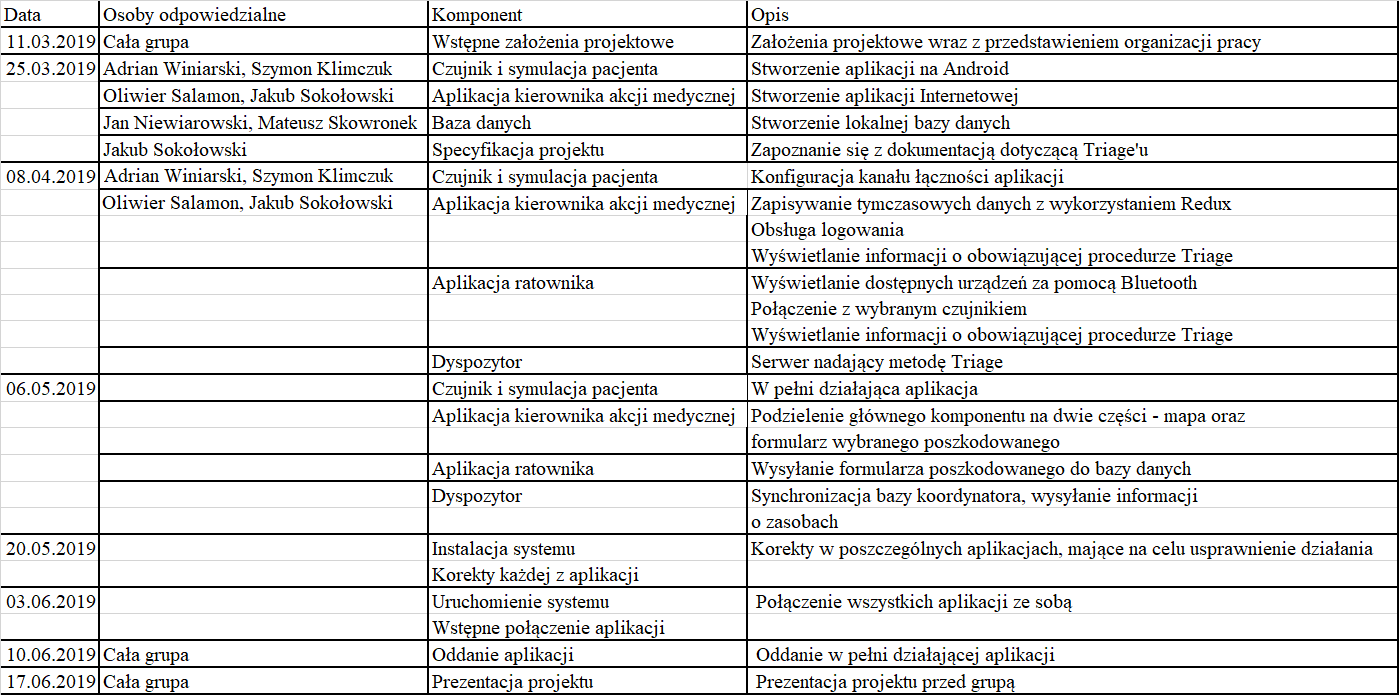
\includegraphics[width=0.95\textwidth]{img/harmonogram.png}
  \caption{Harmonogram pracy} 
  \label{fig:org}                                       
\end{figure}

\section{Specyfikacja}
\subsubsection{25.03.2019}
\subsection{KAM - mapa poszkodowanych}
\subsubsection{Data}
25.03
\subsubsection{Osoby odpowiedzialne}
Oliwier Salamon, Jakub Sokołowski
\subsubsection{Scenariusze}
Aktor: Kierujący Akcją Medyczną
\subsubsection{Scenariusz 1}
Po przejściu na widok "mapa", KAM widzi mapę, na której znajdują się znaczniki reprezentujące lokalizację poszkodowanych.
\subsubsection{Scenariusz 2}
Po kliknięciu na znacznik, po prawej stronie mapy pokaże się panel z danymi pacjenta, zdefiniowanymi przez dokument \textbf{victimInfo}.
\subsubsection{Scenariusz 3}
Po kliknięciu na przycisk "odśwież", z bazy danych pobierane są obecne dane i widok jest odświeżany.
\subsubsection{Specyfikacja}
\begin{itemize}
    \item{Widok "mapa" będzie dostępny tylko po zalogowaniu}
    \item{Dane widoku mapy}
    \item{Do generowania ma zostać API Google Maps}
    \item{Dane są automatycznie odświeżane co 30s}
\end{itemize}
\subsubsection{Wymagania zewnętrzne}
Baza danych z dokumentami \textbf{victimInfo}.

\subsection{Baza danych }
\subsubsection{Data}
25.03.2019
\subsubsection{Osoby odpowiedzialne}
Jan Niewiarowski, Mateusz Skowronek

\subsubsection{Specyfikacja}
Lokalna baza danych została zaimplementowana na silniku MongoDB. Silnik MongoDB jest przykładem bazy niewykorzystującej języka SQL oraz nierelacyjnej. Charakteryzuje się dużą skalowalnością, wydajnością oraz brakiem ściśle zdefiniowanej struktury obsługiwanych baz danych. MongoDB składuje dane w postaci plików JSON, które nazywa dokumentami i umieszcza je w tzw. kolekcjach. Silnik nie wymaga tworzenia schematu bazy danych lecz wstawia dokument JSON do kolekcji, która jeżeli nie istnieje zostaje automatycznie utworzona. 
\newline
W porównaniu z relacyjną bazą danych, np. MySQL, MongoDB jest prostsza i wydajniejszy. Przy użyciu tego silnika można skalować bazę na wiele serwerów.
Dodatkowo bazę można podłączyć i skonfigurować z wieloma różnymi językami programowania, np. Java lub JavaScript.
\newpage

\begin{figure}[h!]
  \centering
    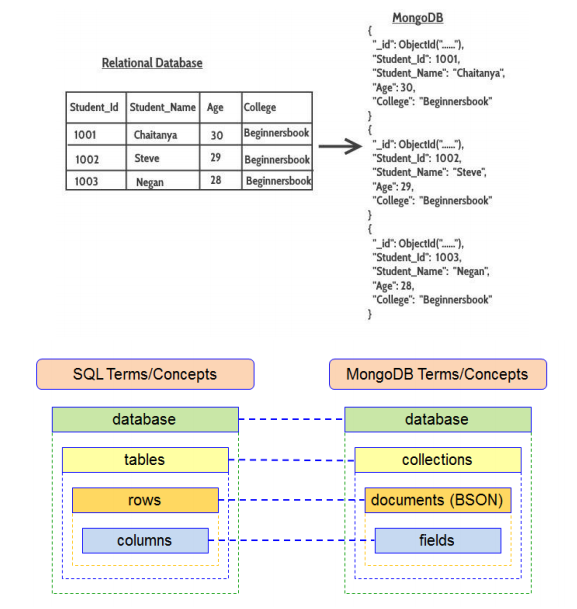
\includegraphics[width=0.95\textwidth]{img/mongo.png}
  \caption{Porównanie relacyjnej bazdy danych z MongoDB} 
  \label{fig:org}                                       
\end{figure}

\newpage

\subsubsection{Kolekcje w bazie danych}
W bazie danych przechowywane będą elementy takie jak: \\
- pomiar czujników (puls i saturacja), \\
- dane poszkodowanego (numer identyfikacyjny, priorytet według zasad triage, lokalizacja, informacje dodatkowe), \\
- informacje konieczne do wypełnienia karty działań kierującego akcją medycznych czynności ratunkowych (KAM), \\
- informacje potrzebne do wypełnienia karty działań dyspozytora medycznego kierującego (DM-K), \\


\subsubsection{Przykładowe kolekcje znajdujące się w bazie}


Dane czujnika:
\begin{verbatim}
sensorInfo = {
    "priority" : enum,
    "lifeFunctionSeries": [
        {
            "timestamp" : unxiTimestamp,
            "pulse":  number,
            "saturation": number,
        }
    ]
}
\end{verbatim}
Dane poszkodowanego:
\begin{verbatim}
victimInfo = {
    "id" : number,
    "priorityHistory": [
        {
            "priorty" : enum,
            "timestamp": unixTimestamp
        }
    ],
    "sensorInfo": sensorInfo,
    "lastKnownCoordinates": GPS,
    "rescueTeamId": string,
    "assignedHospital": string,
    "injuries": string,
    "additionalInfo": string    
}
\end{verbatim}
\newpage
\subsubsection{Karta działań dyspozytora medycznego kierującego (DM-K)}

\begin{figure}[h!]
  \centering
    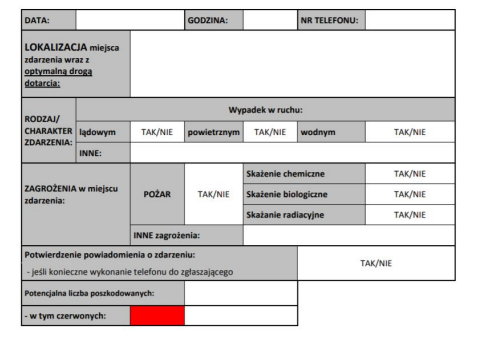
\includegraphics[width=0.95\textwidth]{img/powiadomienia.png}
  \caption{Powiadomienie} 
  \label{fig:org}                                       
\end{figure}

\begin{figure}[h!]
  \centering
    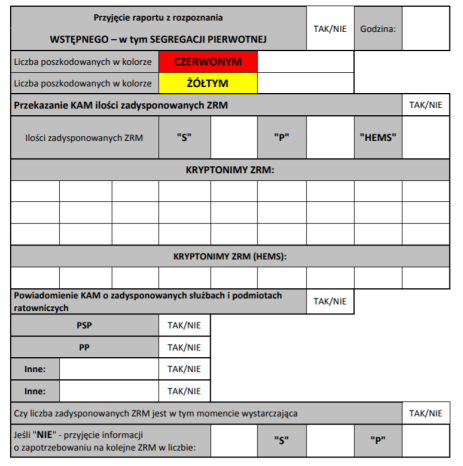
\includegraphics[width=0.95\textwidth]{img/Kamtodmk.png}
  \caption{Wymiana informacji pomiędzy KAM a DM-K} 
  \label{fig:org}                                       
\end{figure}

\begin{figure}[h!]
  \centering
    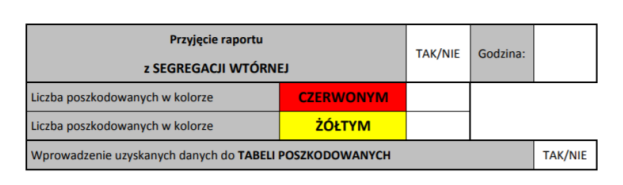
\includegraphics[width=0.95\textwidth]{img/Kamtodmk2.png}
  \caption{Wymiana informacji pomiędzy KAM a DM-K} 
  \label{fig:org}                                       
\end{figure}

\begin{figure}[h!]
  \centering
    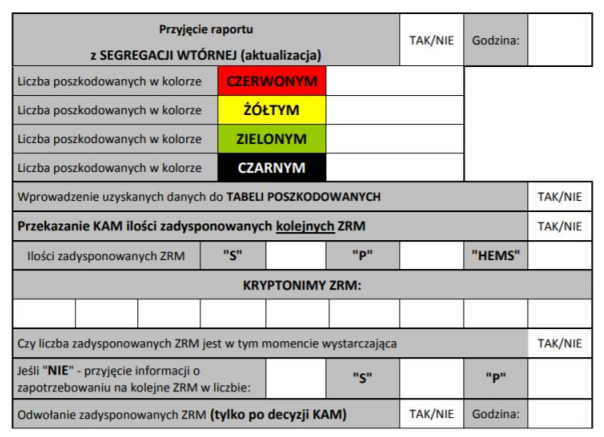
\includegraphics[width=0.95\textwidth]{img/Kamtodmk3.png}
  \caption{Wymiana informacji pomiędzy KAM a DM-K} 
  \label{fig:org}                                       
\end{figure}


\subsection{Aplikacja Poszkodowanego - Symulacja Funkcji Życiowych Pacjenta }
\subsubsection{Data}
25.03
\subsubsection{Osoby odpowiedzialne}
Adrian Winiarski, Szymon Klimczuk

\subsubsection{Specyfikacja}
\begin{itemize}
    \item{Symulowane są 2 funkcje życiowe - puls oraz oddech}
    \item{Sygnały generowane muszą być niezależne od reszty aplikacji}
    \item Generowany sygnał odpowiada stopniowi obrażeń poszkodowanego
\newline
\newline
 Na zdjęciach poniżej są pokazane 3 interfejsy. Na pierwszym mamy interfejs główny. Drugi interfejs z rozwinięta listą w której można skategoryzować pacjenta wybierając odpowiedni kolor do wyboru mamy 4 podstawowe czyli: czarny, czerwony, zielony, żółty.
\begin{figure}[h!]
  \centering
    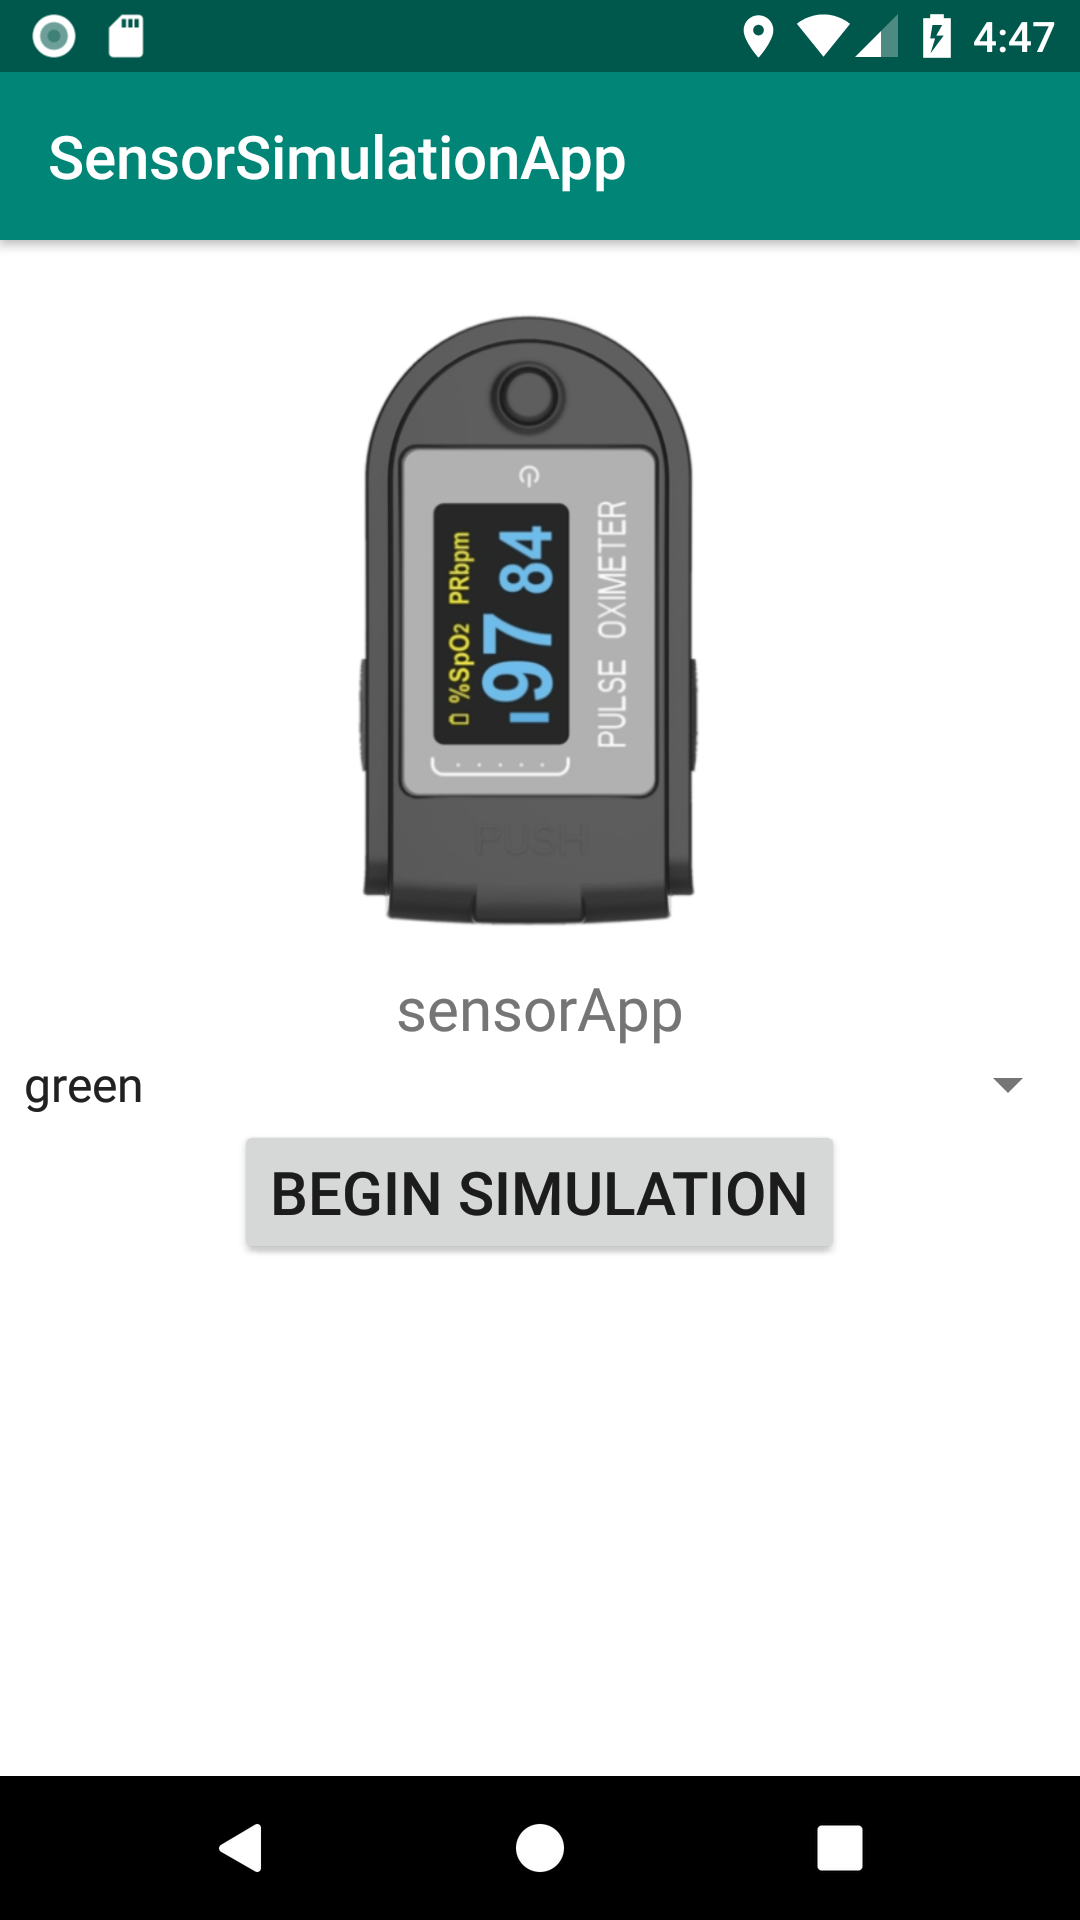
\includegraphics[width=0.30\textwidth]{img/start.png}
  \caption{Główny ekran} 
  \label{fig:org}                                       
\end{figure}
\end{itemize}
\newpage
\begin{figure}[h!]
  \centering
    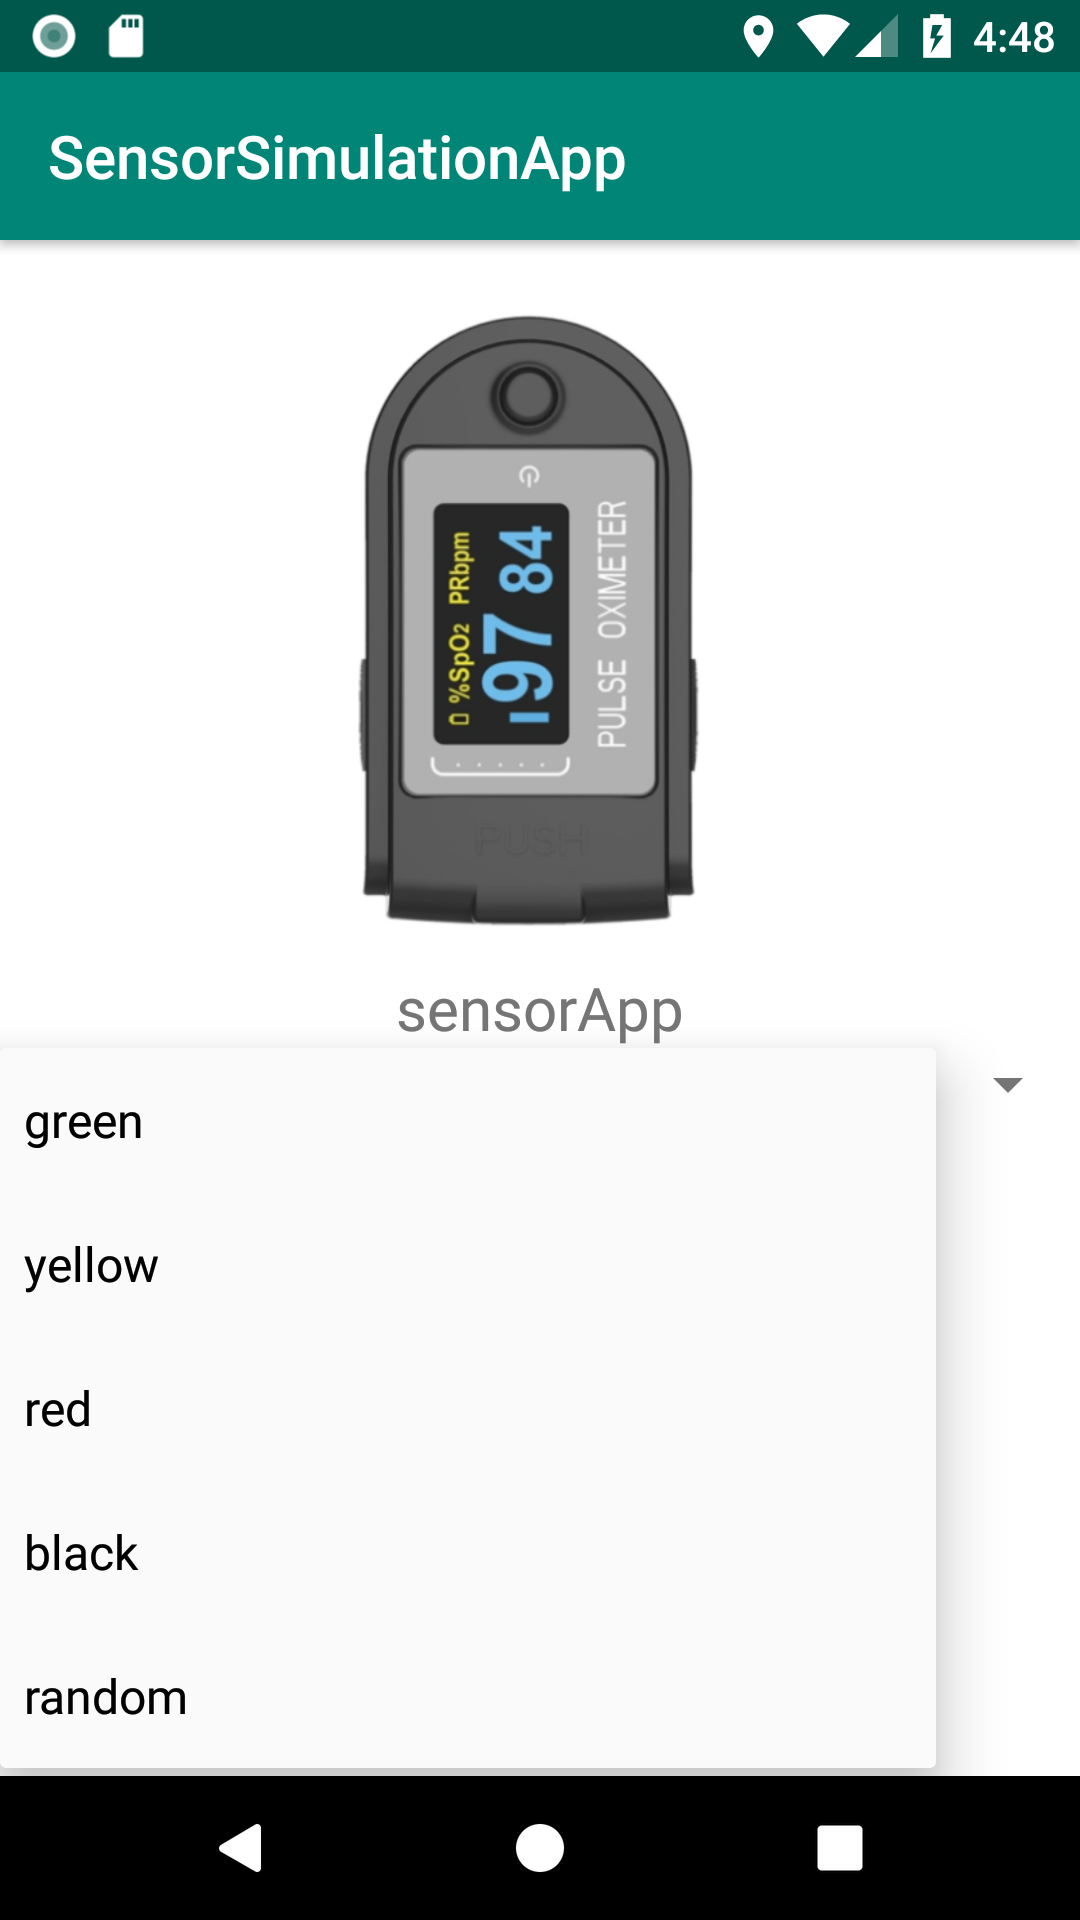
\includegraphics[width=0.30\textwidth]{img/scroll.png}
  \caption{Ekran z rozwiniętą listą} 
  \label{fig:org}                                       
\end{figure}
\begin{figure}[h!]
  \centering
    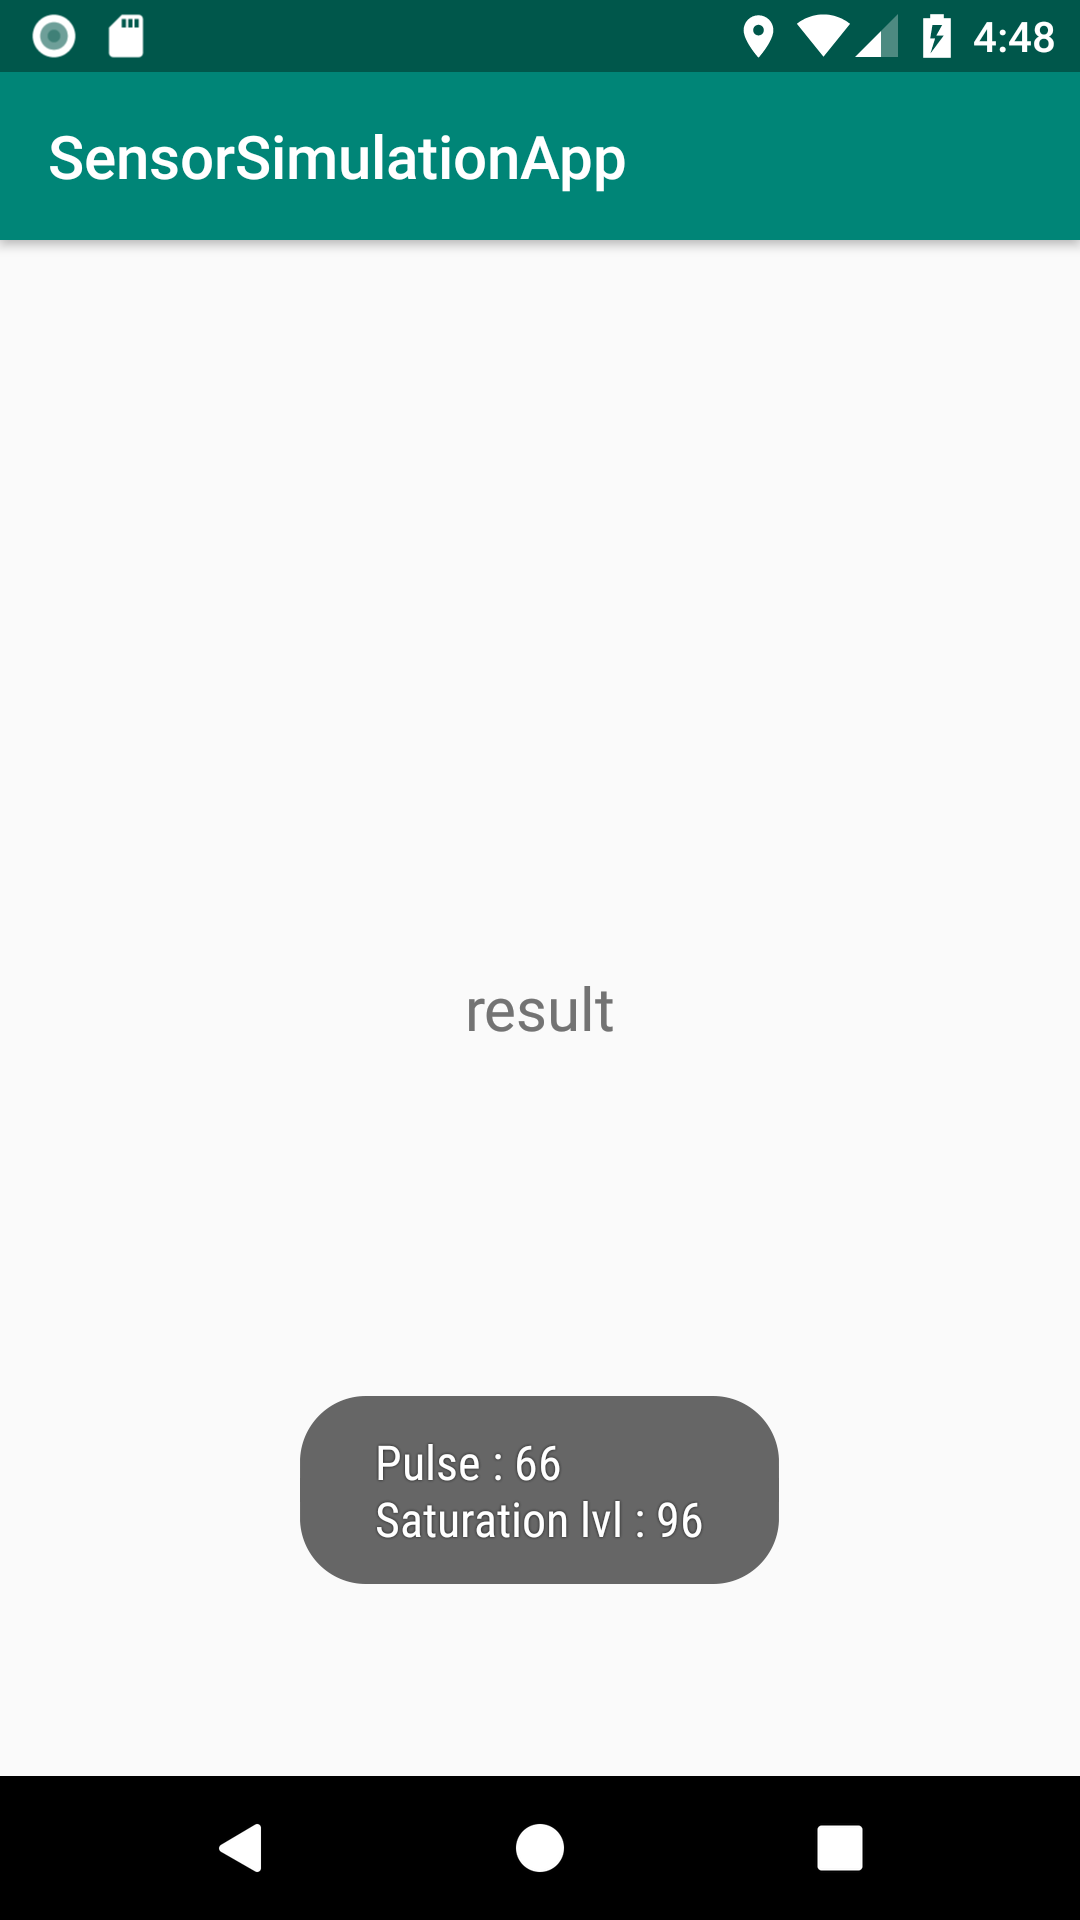
\includegraphics[width=0.30\textwidth]{img/result.png}
  \caption{Ekran z symulowaną saturacją i pulsem} 
  \label{fig:org}                                       
\end{figure}

\subsubsection{Wymagania zewnętrzne}



Dokument sporządził \hspace{1cm} Dokument sprawdził\hspace{1cm} Dokument zatwierdził 
\newline

\begin{thebibliography}{9}
\bibitem{procedury} 
Zespół powołany w dniu 18 czerwca 2014 roku
przez Dyrektora SP ZOZ Lotnicze Pogotowie Ratunkowe
dra n. med. Roberta Gałązkowskiego \\
\textit{Procedury postępowania na wypadek wystąpienia zdarzenia mnogiego/masowego}
\bibitem{sprzet}
Wyposażenie karetek\\
\texttt{https://gloswielkopolski.pl/ten-sprzet-ratuje-zycie-zobacz-jak-sa\\-wyposazone-karetki-poznanskiego-pogotowia-ratunkowego\\-zdjecia/ga/12994592/zd/27833720} [dostep 04-04-2019]
\end{thebibliography}
\begin{appendices}
\chapter{Jakiś Dodatek}
zawartość
\end{appendices}

\end{document}